\chapter{Results}
This chapter present the results of the bachelor thesis. Because a lot of changes influence the simulation but are not observable, only visible results are mentioned in this chapter. These visible results are presented with a voxel density of 1. Therefore \SI{1}{\micro\metre} equals 1 voxel.

\section{Draw sphere cells}
With the created method of section \ref{sec:DrawSphereCells} the program is now able to draw a cell as sphere out of
voxel, as it is displayed in figure \ref{img:DrawnSphereCellRadius5And9} and \ref{img:DrawnSphereCellRadius14And23}. \newline
Since voxels, cuboids, are used in the 3D simulation to draw a cell as a sphere, it is not possible to draw a perfectly round sphere. This problem is displayed with an circle and a square in picture \ref{img:CircleSquarePixels} at page \pageref{img:CircleSquarePixels}. The drawn cells are as spherish as possible in the simulation with the use of voxels. \newline
Figure \ref{img:DrawnSphereCellRadius5And9} displays two independent drawn cells with a radius of \SI{5}{\micro\metre} and \SI{9}{\micro\metre}. These cells show that there are a lot of edges in the sphere. As the radius increases, the sphere shape of the cell gets more detailed, as it is displayed in figure \ref{img:DrawnSphereCellRadius14And23}. In this figure two cells are drawn idepently with a radius of \SI{14}{\micro\metre} and \SI{23}{\micro\metre}. With the increase of the radius, the deviation of the surface increases as well, as it is shown in figure \ref{img:DeviationSphere}. This might be a result as the surface of a sphere and a cuboid, with the daimeter $2 \cdot r$, deviates more as $r$ increases.

\begin{figure}
	\begin{center}
	\subfloat[]{
		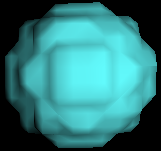
\includegraphics[scale=1.05]{figures/VoxelSphere/Radius5-0.png}
	}
	\subfloat[]{
		\hspace{0.5cm}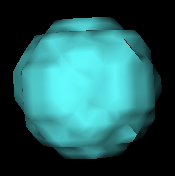
\includegraphics[scale=0.9]{figures/VoxelSphere/Radius5-1.png}
	}
	\end{center}
	\begin{center}
	\subfloat[]{
		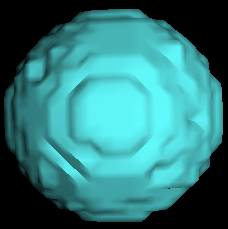
\includegraphics[scale=0.73]{figures/VoxelSphere/Radius9-0.png}
	}
	\subfloat[]{
		\hspace{0.5cm}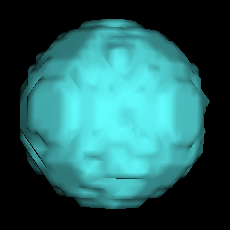
\includegraphics[scale=0.69]{figures/VoxelSphere/Radius9-1.png}
	}
	\end{center}
	\caption{\label{img:DrawnSphereCellRadius5And9}A single cell drawn into the simulation field. The radius of the cell of (a) and (b) is 5 and the radius of the cell of (c) and (d) is 9. Pictures (a) and (c) are with the front view, whereas the
pictures (b) and (d) have an view angle of around 45 degree. The color of the cell is chosen in
a way that more details are visible.}
\end{figure}

\begin{figure}
	\begin{center}
	\subfloat[]{
		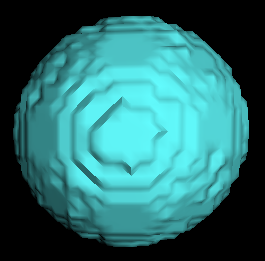
\includegraphics[scale=0.65]{figures/VoxelSphere/Radius14-0.png}
	}
	\subfloat[]{
		\hspace{0.5cm}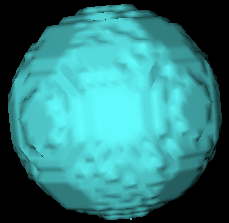
\includegraphics[scale=0.76]{figures/VoxelSphere/Radius14-1.png}
	}
	\end{center}
	\begin{center}
	\subfloat[]{
		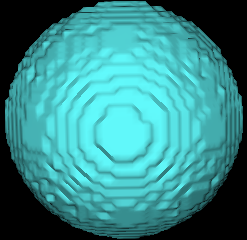
\includegraphics[scale=0.705]{figures/VoxelSphere/Radius23-0.png}
	}
	\subfloat[]{
		\hspace{0.5cm}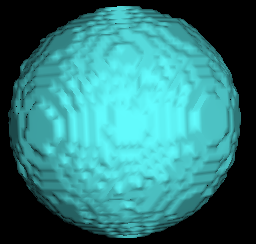
\includegraphics[scale=0.695]{figures/VoxelSphere/Radius23-1.png}
	}
	\end{center}
	\caption{\label{img:DrawnSphereCellRadius14And23}A single cell drawn into the simulation field. The radius of the cell of (a) and (b) is 14 and the radius of the cell of (c) and (d) is 23. Pictures (a) and (c) are with the front view, whereas the
pictures (b) and (d) have an view angle of around 45 degree. The color of the cell is chosen in
a way that more details are visible.}
\end{figure}

\newpage
\section{Grow sphere cells}
In section \ref{sec:GrowSphereCell} the factor for the calculation of the surface of the cell was evidenced best to be $1.5$. With this factor it should be possible to let the sphere cell grow as a sphere. To test the growth of the cell, one single cell was placed in the simulation field. As the cell growed during the simulation the volume and surface values were rad out of the command line and compared to the documented values of a drawn cell. \newline
To let a cell grow as a sphere does not work. Even the volume and surface values, calculated by \ac{CC3D}, and the target volume and target surface values, calculated by the program, meet the values of drawn sphere cells with a small deviation \textit{of an maximum deviation up to 50}.

Figures \ref{img:GrowthSphereCellRadius5} and \ref{img:GrowthSphereCellRadius9} display two examples of a single cell placed in the simulation field. It is observable that drawn sphere cells with a smaller radius become a cubish shape faster. In fiugre \ref{img:GrowthSphereCellRadius5} the cell has a cubish form after 50 \ac{MCS} where the cell in figure \ref{img:GrowthSphereCellRadius9} becomes cubish after 750 \ac{MCS}. This might be a result that the larger sphere cell has more detail than the cell with a smaller radius.

\begin{figure}
	\begin{center}
	\subfloat[]{
		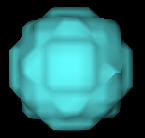
\includegraphics[scale=1.15]{figures/GrowthSphereCell/Radius5/Radius5-MCS0.png}
	}
	\subfloat[]{
		\hspace{0.5cm}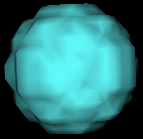
\includegraphics[scale=1.15]{figures/GrowthSphereCell/Radius5/Radius5-MCS0-1.png}
	}
	\end{center}
	\begin{center}
	\subfloat[]{
		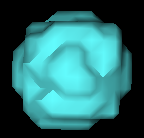
\includegraphics[scale=1.16]{figures/GrowthSphereCell/Radius5/Radius5-MCS50.png}
	}
	\subfloat[]{
		\hspace{0.5cm}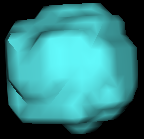
\includegraphics[scale=1.155]{figures/GrowthSphereCell/Radius5/Radius5-MCS50-1.png}
	}
	\end{center}
	\begin{center}
	\subfloat[]{
		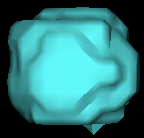
\includegraphics[scale=1.145]{figures/GrowthSphereCell/Radius5/Radius5-MCS250.png}
	}
	\subfloat[]{
		\hspace{0.53cm}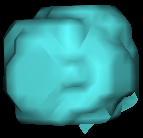
\includegraphics[scale=1.105]{figures/GrowthSphereCell/Radius5/Radius5-MCS250-1.png}
	}
	\end{center}
	\caption{\label{img:GrowthSphereCellRadius5}A sphere cell, with a radius of \SI{5}{\micro\metre} and a voxel density of 1, as it grows. Images (a), (c) and (e) are the front view of the cell and figures (b), (d) and(f) have around a 45 degree angle of the front. Figure (a) and (b) are at \ac{MCS} 0, images (c) and (d) at calculation step 50 and figures (e) and (f) present \ac{MCS} 250.}
\end{figure}

\begin{figure}
	\begin{center}
	\subfloat[]{
		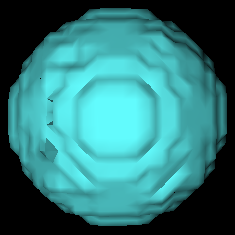
\includegraphics[scale=0.7]{figures/GrowthSphereCell/Radius9/Radius9-MCS0.png}
	}
	\subfloat[]{
		\hspace{0.5cm}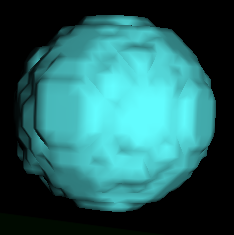
\includegraphics[scale=0.7]{figures/GrowthSphereCell/Radius9/Radius9-MCS0-1.png}
	}
	\end{center}
	\begin{center}
	\subfloat[]{
		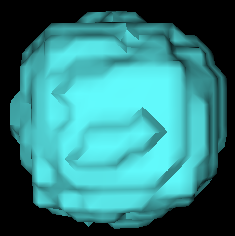
\includegraphics[scale=0.7]{figures/GrowthSphereCell/Radius9/Radius9-MCS750.png}
	}
	\subfloat[]{
		\hspace{0.5cm}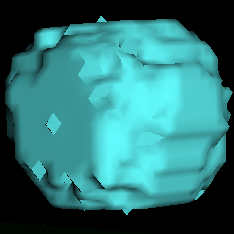
\includegraphics[scale=0.64]{figures/GrowthSphereCell/Radius9/Radius9-MCS750-1.png}
	}
	\end{center}
	\begin{center}
	\subfloat[]{
		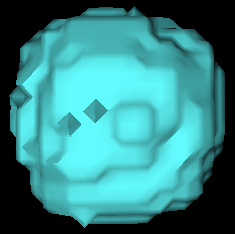
\includegraphics[scale=0.7]{figures/GrowthSphereCell/Radius9/Radius9-MCS1250.png}
	}
	\subfloat[]{
		\hspace{0.5cm}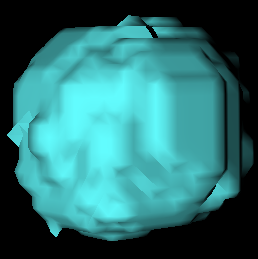
\includegraphics[scale=0.64]{figures/GrowthSphereCell/Radius9/Radius9-MCS1250-1.png}
	}
	\end{center}
	\caption{\label{img:GrowthSphereCellRadius9}A sphere cell, with a radius of \SI{9}{\micro\metre} and a voxel density of 1, as it grows. Images (a), (c) and (e) are the front view of the cell and figures (b), (d) and(f) have around a 45 degree angle of the front. Figure (a) and (b) are at \ac{MCS} 0, images (c) and (d) at calculation step 750 and figures (e) and (f) present \ac{MCS} 1250.}
\end{figure}

\section{Simulations}
Since no simulations are completed with three dimensions, several 3D simulations are presented. The models, which are simulated, are the most realistic models which were evidenced in an earlier version of the project \cite{Torelli2017}. The specific models are...